\documentclass{scrartcl}
\usepackage[utf8]{inputenc}
\usepackage{amsmath}
\usepackage{amssymb}
\usepackage{graphicx}
\usepackage{hyperref}

%opening
\title{Assignment 1}
\author{Daan Spijkers, s1011382\\ Tomás Catalán López, s1081589\\ Willem Lambooy, s1009584}

\begin{document}

\maketitle
Note: you can find the github repository at
\url{github.com/dspijkers/nacu}.

\section{}
Schemata A1 has more wildcards than A2: $o(A1) < o(A2)$. Since both schemata have the same amount of bits, the chance of a non-wildcard bit flipping in A1 is less than the chance of that happening in A2.

Mathematically, this can be computed as follows (with $p_m=0.01$):
\begin{itemize}
  \item Probability of a bit not being flipped after mutation: $1-p_m=0.99$.
  \item Probability that A1 survives: $S_m(A1)=(1-p_m)^{o(A1)}=0.99^4\approx0.961$.
  \item Probability that A2 survives: $S_m(A2)=(1-p_m)^{o(A2)}=0.99^5\approx0.951$.
\end{itemize}

\section*{7}
% the question says function, terminal set AND s-expression, but
% s-expression is just the function and terminal set, no? I'm not sure if
% I'm leaving something out, but I feel like this is fine -- daan
\begin{itemize}
  \item[(a)]
    $T = \{x, y, z, \text{true}, \text{false}\}$. False isn't
    \emph{strictly} necessary, but otherwise it would be a trivial
    formula.

    $F = \{\land, \lor, \leftrightarrow\}$. These all have arity 2.

  \item[(b)]
    $T = \mathbb{R} \cup \{x, z\}$. Technically $0.234$ and $0.789$ are in
    $\mathbb{Q}$, so that would suffice, but taking the reals is more
    standard.

    $F = \{+, -, *\}$. These all have arity 2.

\end{itemize}

\section*{8}
We used the DEAP python framework. Any individuals with errors (so, if it
tried to divide by 0, or log -1) were given fitness $-\infty$. For the
implementation see \emph{8/code.py}, and to generate the plots simply run
\emph{8/plots.py}. (both in the github repository linked at the start of
this file)

\begin{figure}
  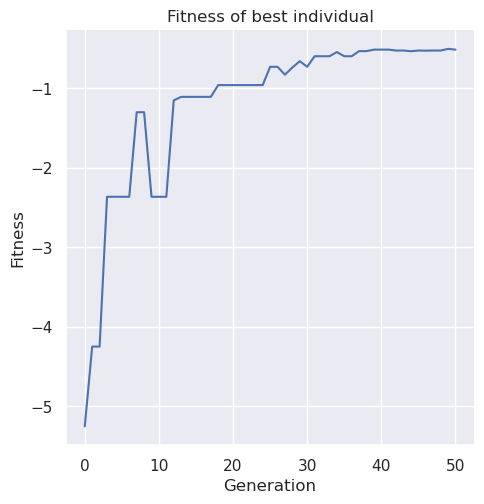
\includegraphics[width=0.5\textwidth]{8/score_best}

  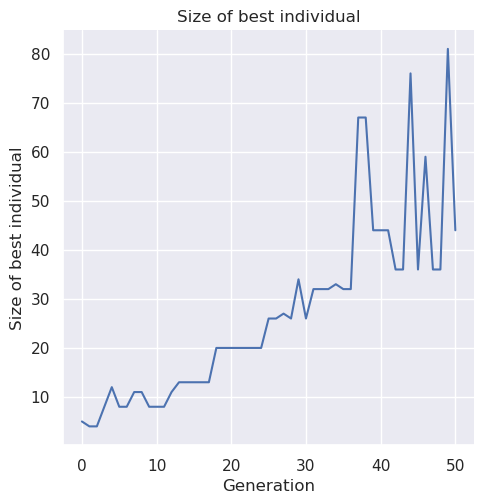
\includegraphics[width=0.5\textwidth]{8/size_best}

  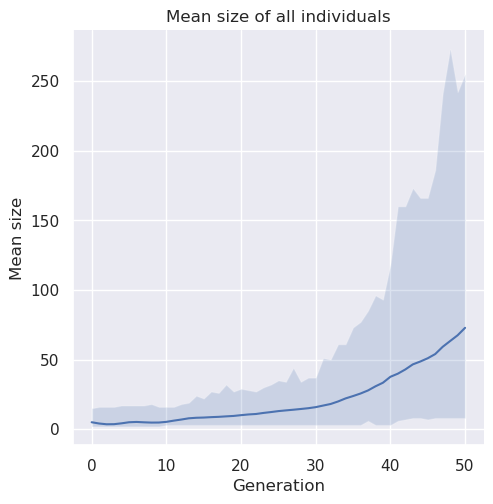
\includegraphics[width=0.5\textwidth]{8/mean_size}
\end{figure}

%TODO: maybe add a proper reference using a reference manager.
We do in fact see a undesirable phenomenon: bloat. Two techniques to
prevent this are given in the Javed, Noman, and Fermand Gobet paper, which
is also referenced in the lecture slides (page 47).

These techniques are generationwide simplification (gws) and pruning. In
gws every kth generation (for some k) we simplify the trees. Instead of
producing offspring from mutation or crossover, we generate offspring by
selecting subtrees.

Pruning is a similar idea, but instead of doing it populationwide, we pick
the top few percent fittest individuals, and replace them by the fittest
out of some generated set of subtrees.

\end{document}
